% Classes of src/core/Math/Integral and their dependencies. Paper: section "Interpolation, integration and
% differentiation" (fig:integral); Doxygen: Integrator.hpp.
%   pdflatex IntegralClasses.tex; pdftoppm -r 200 -png -singlefile IntegralClasses.pdf IntegralClasses;
%   pdftocairo -svg IntegralClasses.pdf IntegralClasses.svg
\documentclass[tikz,border=2pt]{standalone}
% Shared style of the class diagrams of CAP (figures/*Classes.tex): \input after \documentclass[tikz]{standalone}.
%  - boxes: blue = abstract base class, light blue = class, green = entry class of the folder (steering class, task),
%    yellow = free functions (tools), grey = class of another folder;
%  - arrows: open triangle = inherits from; dashed with diamond = owns (holds); dashed with arrow = uses.
\usepackage[scaled=0.92]{helvet}
\usetikzlibrary{arrows.meta,shapes.multipart,positioning,fit,backgrounds,calc}
\renewcommand{\familydefault}{\sfdefault}
\definecolor{abstract}{HTML}{D6E4F5}
\definecolor{concrete}{HTML}{EEF4FB}
\definecolor{steer}{HTML}{DCEFD9}
\definecolor{tools}{HTML}{FFF8E6}
\definecolor{external}{HTML}{E9E9E9}
\definecolor{dependline}{HTML}{8A6D3B}
\definecolor{folder}{HTML}{F7F7F7}
\tikzset{
  every picture/.style={font=\scriptsize},
  cls/.style={draw, fill=concrete, align=center, inner sep=2.5pt, text width=#1, font=\tiny},
  cls/.default=3.0cm,
  abs/.style={cls=#1, fill=abstract},
  abs/.default=3.0cm,
  steer/.style={cls=#1, fill=steer, line width=0.8pt},
  steer/.default=4.2cm,
  tool/.style={cls=#1, fill=tools},
  tool/.default=4.2cm,
  ext/.style={cls=#1, fill=external, dashed},
  ext/.default=2.6cm,
  fam/.style={draw, rectangle split, rectangle split parts=2, rectangle split part fill={#1,white},
              rectangle split part align={center,left}, inner sep=2.5pt, align=left},
  inherit/.style={-{Triangle[open,length=2.2mm,width=2.2mm]}, thin},
  uses/.style={dashed, dependline, -{Stealth[length=1.6mm]}, thin},
  owns/.style={dashed, dependline, {Diamond[length=2.4mm,width=1.6mm]}-, thin},
  lbl/.style={font=\tiny, text=dependline, align=center},
  note/.style={font=\tiny, align=left, text=black!70},
  title/.style={font=\footnotesize\bfseries, anchor=north west},
}
% a member line in a class box
\newcommand{\m}[1]{\\#1}
\newcommand{\cn}[1]{{\scriptsize\textbf{#1}}}
\newcommand{\an}[1]{{\scriptsize\textbf{\textit{#1}}}}

% legend common to the class diagrams (place with \legendat{x}{y})
\newcommand{\legendat}[2]{%
  \begin{scope}[shift={(#1,#2)}, font=\tiny]
    \node[abs=0.9cm, minimum height=3mm, inner sep=1pt] (lA) at (0,0) {abstract};
    \node[cls=0.9cm, minimum height=3mm, inner sep=1pt, right=1mm of lA] (lC) {class};
    \node[steer=1.1cm, minimum height=3mm, inner sep=1pt, right=1mm of lC] (lS) {entry class};
    \node[tool=1.1cm, minimum height=3mm, inner sep=1pt, right=1mm of lS] (lT) {functions};
    \node[ext=1.3cm, minimum height=3mm, inner sep=1pt, right=1mm of lT] (lE) {other folder};
    \draw[inherit] ($(lE.east)+(1mm,0)$) -- ++(5mm,0) node[right, inner sep=1pt] (l1) {inherits};
    \draw[owns] ($(l1.east)+(1mm,0)$) -- ++(5mm,0) node[right, inner sep=1pt] (l2) {owns};
    \draw[uses] ($(l2.east)+(1mm,0)$) -- ++(5mm,0) node[right, inner sep=1pt] {uses};
  \end{scope}}

\begin{document}
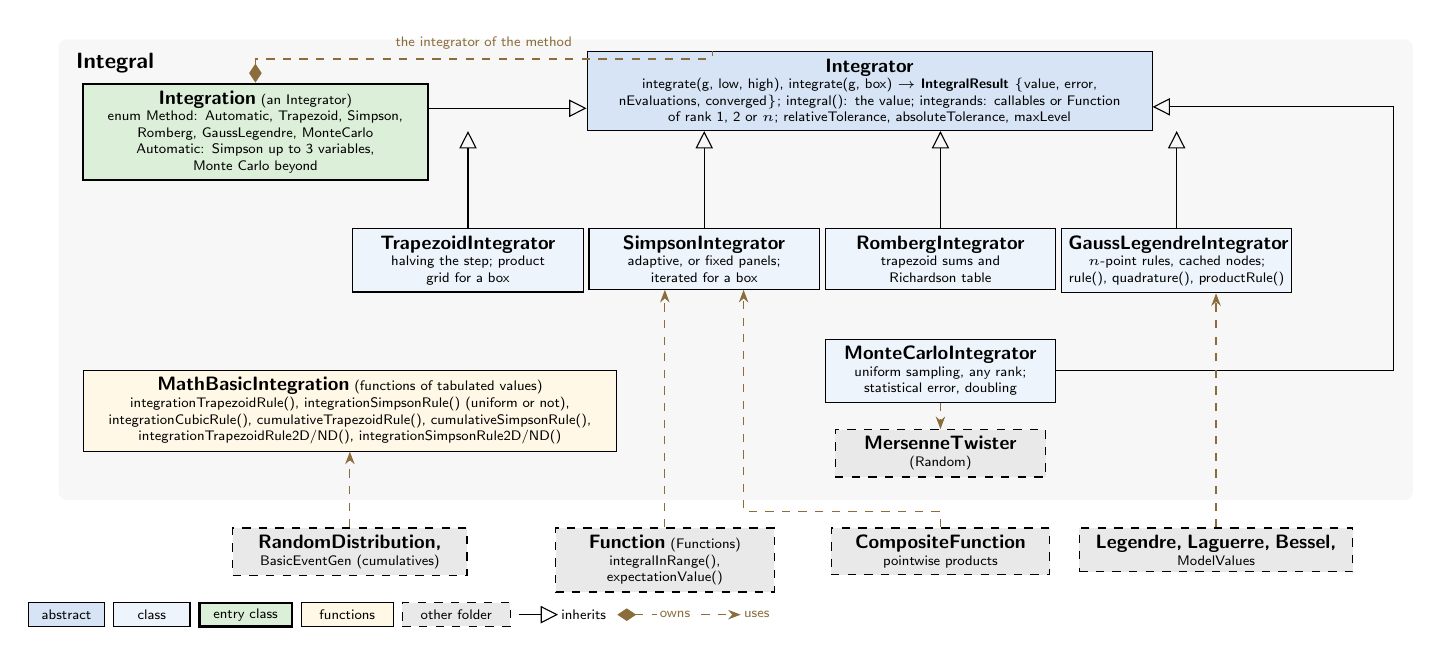
\begin{tikzpicture}[every node/.append style={anchor=north}]
  \begin{scope}[on background layer]
    \fill[folder, rounded corners=3pt] (-0.1,-0.2) rectangle (17.1,-6.05);
  \end{scope}
  \node[title] at (0.0,-0.25) {Integral};

  \node[abs=7.0cm] (Integrator) at (10.2,-0.35)
    {\an{Integrator}\m{integrate(g, low, high), integrate(g, box) $\to$ \textbf{IntegralResult} \{value, error,}
     \m{nEvaluations, converged\}; integral(): the value; integrands: callables or Function}
     \m{of rank 1, 2 or $n$; relativeTolerance, absoluteTolerance, maxLevel}};
  \node[steer=4.2cm] (Integration) at (2.4,-0.75)
    {\cn{Integration} \tiny(an Integrator)\m{enum Method: Automatic, Trapezoid, Simpson,}
     \m{Romberg, GaussLegendre, MonteCarlo}\m{Automatic: Simpson up to 3 variables,}\m{Monte Carlo beyond}};

  \node[cls=2.75cm] (Trap) at (5.1,-2.6) {\cn{TrapezoidIntegrator}\m{halving the step; product}\m{grid for a box}};
  \node[cls=2.75cm] (Simp) at (8.1,-2.6) {\cn{SimpsonIntegrator}\m{adaptive, or fixed panels;}\m{iterated for a box}};
  \node[cls=2.75cm] (Romb) at (11.1,-2.6) {\cn{RombergIntegrator}\m{trapezoid sums and}\m{Richardson table}};
  \node[cls=2.75cm] (GL) at (14.1,-2.6) {\cn{GaussLegendreIntegrator}\m{$n$-point rules, cached nodes;}\m{rule(), quadrature(), productRule()}};
  \node[cls=2.75cm] (MC) at (11.1,-4.0) {\cn{MonteCarloIntegrator}\m{uniform sampling, any rank;}\m{statistical error, doubling}};
  \node[ext=2.5cm] (Random) at (11.1,-5.15) {\cn{MersenneTwister} \tiny(Random)};
  \foreach \c in {Trap,Simp,Romb,GL} \draw[inherit] (\c.north) -- (\c.north |- Integrator.south);
  \draw[inherit] (MC.east) -- (16.85,0 |- MC.east) |- ([yshift=-2mm]Integrator.east);
  \draw[inherit] ([yshift=3mm]Integration.east) -- ([yshift=3mm]Integration.east -| Integrator.west);
  \draw[owns] (Integration.north) -- ++(0,0.3) -| node[lbl, pos=0.25, above]{the integrator of the method} ([xshift=-2.0cm]Integrator.north);
  \draw[uses] (MC.south) -- (Random.north);

  \node[tool=6.6cm] (Basic) at (3.6,-4.4)
    {\cn{MathBasicIntegration} \tiny(functions of tabulated values)\m{integrationTrapezoidRule(), integrationSimpsonRule() (uniform or not),}
     \m{integrationCubicRule(), cumulativeTrapezoidRule(), cumulativeSimpsonRule(),}
     \m{integrationTrapezoidRule2D/ND(), integrationSimpsonRule2D/ND()}};

  % users
  \node[ext=2.8cm] (RD) at (3.6,-6.4) {\cn{RandomDistribution,}\m{BasicEventGen (cumulatives)}};
  \node[ext=2.6cm] (Function) at (7.6,-6.4) {\an{Function} \tiny(Functions)\m{integralInRange(), expectationValue()}};
  \node[ext=2.6cm] (Comp) at (11.1,-6.4) {\cn{CompositeFunction}\m{pointwise products}};
  \node[ext=3.3cm] (Ortho) at (14.6,-6.4) {\cn{Legendre, Laguerre, Bessel,}\m{ModelValues}};
  \draw[uses] (RD.north) -- (Basic.south);
  \draw[uses] (Function.north) -- (Function.north |- Simp.south);
  \draw[uses] (Comp.north) -- ++(0,0.2) -| ([xshift=0.5cm]Simp.south);
  \draw[uses] (Ortho.north) -- (Ortho.north |- GL.south);
  \legendat{0.0}{-7.35}
\end{tikzpicture}
\end{document}
